\subsubsection{Listar}

  \paragraph{}Para mostrar esta lista, es necesario establecer el centro para
  el que mostrar los administradores de centro disponibles. Para ello, habrá
  que elegir el centro en la lista desplegable que se muestra en la figura
  \ref{capturaPantallaSelectCentro}.

  \begin{figure}[!ht]
    \begin{center}
      \fbox{
      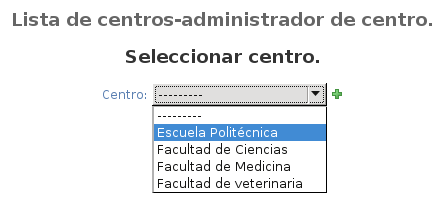
\includegraphics[scale=0.55]{4.Funcionamiento_Aplicacion/4.3.Gestion/4.3.1.Administrador_Principal/4.3.1.4.Centro_AdministradorCentro/select_centro.png}
      }
      \caption{Captura de pantalla de la lista desplegable para seleccionar centro para el usuario \textit{Administrador principal}.}
      \label{capturaPantallaSelectCentro}
    \end{center}
  \end{figure}

  \paragraph{}Nótese que si no existieran elementos disponibles en el sistema,
  la lista desplegable aparecería vacía. Por tanto, se proporciona al usuario
  un icono, representado por una cruz verde, para añadir nuevos elementos al
  sistema. Este icono es el mostrado en la figura \ref{capturaBotonAdd}. Al
  pulsar dicho botón, aparecerá la ventana de creación de un nuevo elemento.

  \begin{figure}[!ht]
    \begin{center}
      \fbox{
      
\includegraphics[scale=0.55]{4.Funcionamiento_Aplicacion/4.3.Gestion/4.3.1.Administrador_Principal/4.3.1.1.Introduccion/botonAdd.png}
      }
      \caption{Captura de pantalla del botón \textit{Añadir}.}
      \label{capturaBotonAdd}
    \end{center}
  \end{figure}

  \paragraph{}Una vez seleccionado el centro, se muestra la lista completa de
  centro - administradores de centro que aparecen en el sistema. La figura
  \ref{capturaPantallaListaCentroAdministradoresCentroAdminPrincipal} muestra
  una captura de pantalla de la lista de centro - administradores de centro.

  \begin{figure}[!ht]
    \begin{center}
      \fbox{
      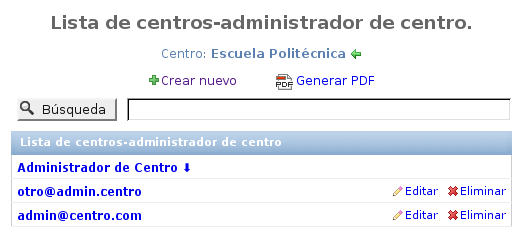
\includegraphics[scale=0.55]{4.Funcionamiento_Aplicacion/4.3.Gestion/4.3.1.Administrador_Principal/4.3.1.4.Centro_AdministradorCentro/lista_centro_adminCentro.png}
      }
      \caption{Captura de pantalla de la lista de centro - administradores de centro para el usuario \textit{Administrador principal}.}
      \label{capturaPantallaListaCentroAdministradoresCentroAdminPrincipal}
    \end{center}
  \end{figure}

  \paragraph{}Si se quisiera refinar el listado de elementos mostrados, es
  posible seleccionar nuevos parámetros pulsando el icono \textit{Seleccionar}
  que aparece al lado de cada elemento. Este icono aparece en la figura
  \ref{capturaBotonSeleccionar}.

  \begin{figure}[!ht]
    \begin{center}
      
\includegraphics[scale=0.55]{4.Funcionamiento_Aplicacion/4.3.Gestion/4.3.1.Administrador_Principal/4.3.1.1.Introduccion/botonSeleccionar.png}
      \caption{Captura de pantalla del botón \textit{Seleccionar}.}
      \label{capturaBotonSeleccionar}
    \end{center}
  \end{figure}
